\documentclass{beamer}
	
	\mode<presentation>
	{
		\usetheme{Madrid}
		\usecolortheme{default}
		\usefonttheme{serif}
		\setbeamertemplate{navigation symbols}{}
		\setbeamertemplate{caption}[numbered]
	
	\makeatother
	\setbeamertemplate{footline}
	{
	  \leavevmode%
	  \hbox{%
	  \begin{beamercolorbox}[wd=.4\paperwidth,ht=2.25ex,dp=1ex,center]{author in head/foot}%
	    \usebeamerfont{author in head/foot}\insertshortauthor
	  \end{beamercolorbox}%
	  \begin{beamercolorbox}[wd=.6\paperwidth,ht=2.25ex,dp=1ex,center]{title in head/foot}%
	    \usebeamerfont{title in head/foot}\insertshorttitle\hspace*{16em}
	    \insertframenumber{} / \inserttotalframenumber\hspace*{1ex}
	  \end{beamercolorbox}}%
	  \vskip0pt%
	}
	\makeatletter
	
	}
	
	\usepackage[french]{babel}
	\usepackage[utf8x]{inputenc}
	\usepackage{comment}
	\usepackage{graphicx}
	\usepackage{multimedia}
	
	\newcommand{\colorized}[1]{{\color{red}{#1}}}
	
	
	% Presentation informations
	\title{Audit et sécurité web}
	\author{Pierre-Marie JUNGES, Florent NOSARI}
	\institute[UL] {
		Université de Lorraine \\
	}
	
	\date{\today}
	
% Pima: intro - Partie 1, 3 - conclusion
% Florent: Partie 2

	\begin{document}
	
\setbeamertemplate{headline}{}
\begin{frame}
	\titlepage 
\end{frame}
	
\begin{frame}{Introduction}
	\begin{itemize}
		\item Sécuriser une application web $\rightarrow$ enjeu important
		\item Application indéfiniment invulnérable $\rightarrow$ impossible
		\item Vérifier régulièrement le niveau de sécurité $\rightarrow$ audit
	\end{itemize}
	$\newline$
	\centering
	$\rightarrow$ Audit de sécurité d'une application web
\end{frame}
	
\begin{frame}{Plan}
	\tableofcontents
\end{frame}

\begin{frame}{Termes et definitions}
	\begin{block}{Audit de sécurité}
		\begin{itemize}
			\item Vue à un instant T de la sécurité d'un système
			\item Pratique encadré (lois, réglementations, normes ISO 19011/27001)
			\item Objectif d'identifier et d'évaluer de potentiels vulnérabilités
			\item Établir des recommendations, corrections
		\end{itemize}
	\end{block}
	\begin{block}{Auditeur}
		Personne participante à la réalisation d'un audit
	\end{block}
	\begin{block}{Audité}
		Commanditaire de l'audit
	\end{block}
\end{frame}


\section{Initier l'audit}

\subsection{Mise en place}
\begin{frame}{Mise en place}
	Contact audité-auditeur : 
	\begin{itemize}
		\item Objectif
		\item Porté 
		\item Méthodes (boite blanche/grise/noire) 
		\item Demandes techniques et administratives 
		\item Définition des échéances 
		\item Composition de l'équipe 
		\item Confirmation légale 
	\end{itemize}		
\end{frame}
\begin{frame}{Mise en place}
	Contact audité-auditeur : 
	\begin{itemize}
		\item Objectif \\
		      $\rightarrow$ \colorized{vérifier des vulnérabilités de l'OWASP TOP 10}
		\item Porté \\
		      $\rightarrow$ \colorized{application web DVWA (en local)}
		\item Méthodes (boite blanche/grise/noire) \\
		      $\rightarrow$ \colorized{boite blanche}
		\item Demandes techniques et administratives \\
		      $\rightarrow$ \colorized{code source}
		\item Définition des échéances \\
		      $\rightarrow$ \colorized{\today}
		\item Composition de l'équipe 
		\item Confirmation légale 
	\end{itemize}		
\end{frame}

\begin{frame}{OWASP ?}
	\begin{block}{OWASP}
		\begin{itemize}
			\item Organisation internationale
			\item Spécialisée en sécurité des applications Web
			\item Fournie des informations sur des failles de sécurité  
		\end{itemize}	
	\end{block}
	$\newline$
	Top 10 $\rightarrow$ 80-90\% des attaques/menaces (2017)
	$\newline$
	\begin{block}{Vulnérabilités à vérifier}
		\begin{enumerate}
			\item Injection
			\item Violation de gestion d'authentification et de session
			\item Cross-Site Scripting (XSS) 
		\end{enumerate}
	\end{block}
\end{frame}

\subsection{Activités d'audit}
\begin{frame}{Activités d'audit}
	Suivant les objectifs  définis, on choisit une/des méthode(s) d'audit
	\begin{itemize}
		\item Audit organisationnel
		\item Tests d'intrusion 			
		\item Revue de code source
		\item Relevés de configuration
		\item Analyse d'architecture	
	\end{itemize}
\end{frame}
\begin{frame}{Méthodes d'audit choisies}
	"Audit applicatif" recommandé par l'ANSSI:
	\begin{itemize}
		\item Revue de code source
		\item Relevés de configuration
	\end{itemize}
	$\newline$
	+ Tests d'intrusion
	$\newline$
	$\newline$
	\colorized{L'ANSSI recommande de ne jamais faire uniquement les tests d'intrusion}
\end{frame}

\section{Execution de l'audit}	
\subsection{Outils utilisés} 
\begin{frame}{Outils utilisés}
	\begin{figure}
		\centering
		\begin{minipage}{.3\textwidth}
			\centering
			
\includegraphics[width=.4\linewidth]{schemas/images/w3af.png}
			\break
			w3af
		\end{minipage}%
		\begin{minipage}{.3\textwidth}
			\centering
			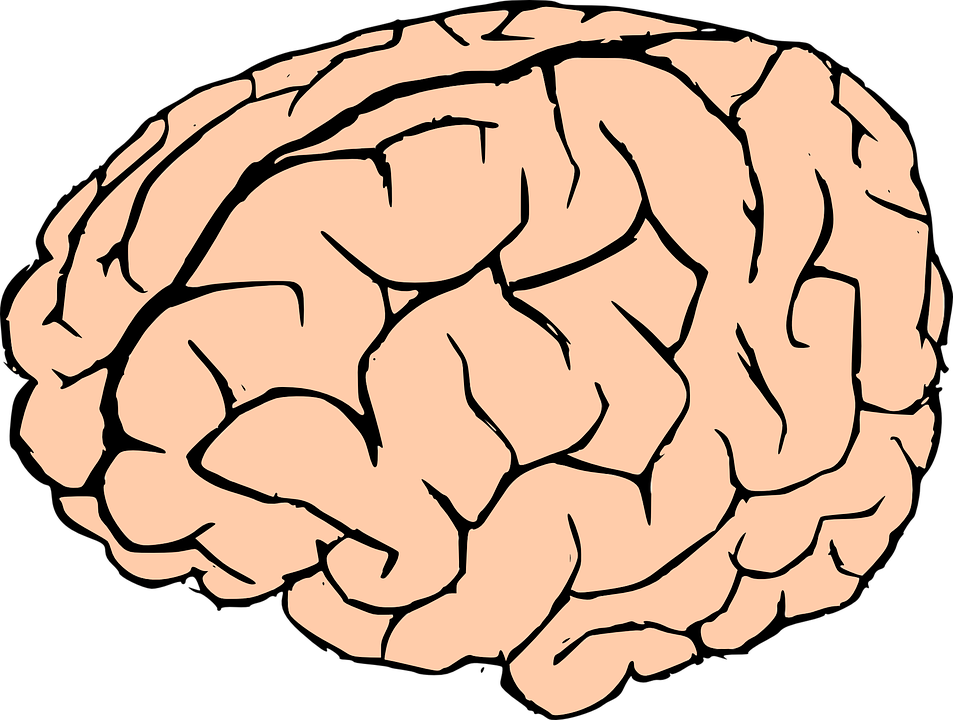
\includegraphics[width=.4\linewidth]{schemas/images/brain.png}
			\break 
			Raisonnement humain
		\end{minipage}
		\begin{minipage}{.3\textwidth}
			\centering
			
\includegraphics[width=.4\linewidth]{schemas/images/zap.png}
			\break 
			OWASP Zap
		\end{minipage}
	\end{figure}	
\end{frame}

\subsection{Tests d'intrusion}
\begin{frame}{Injection (OS)}
\centering
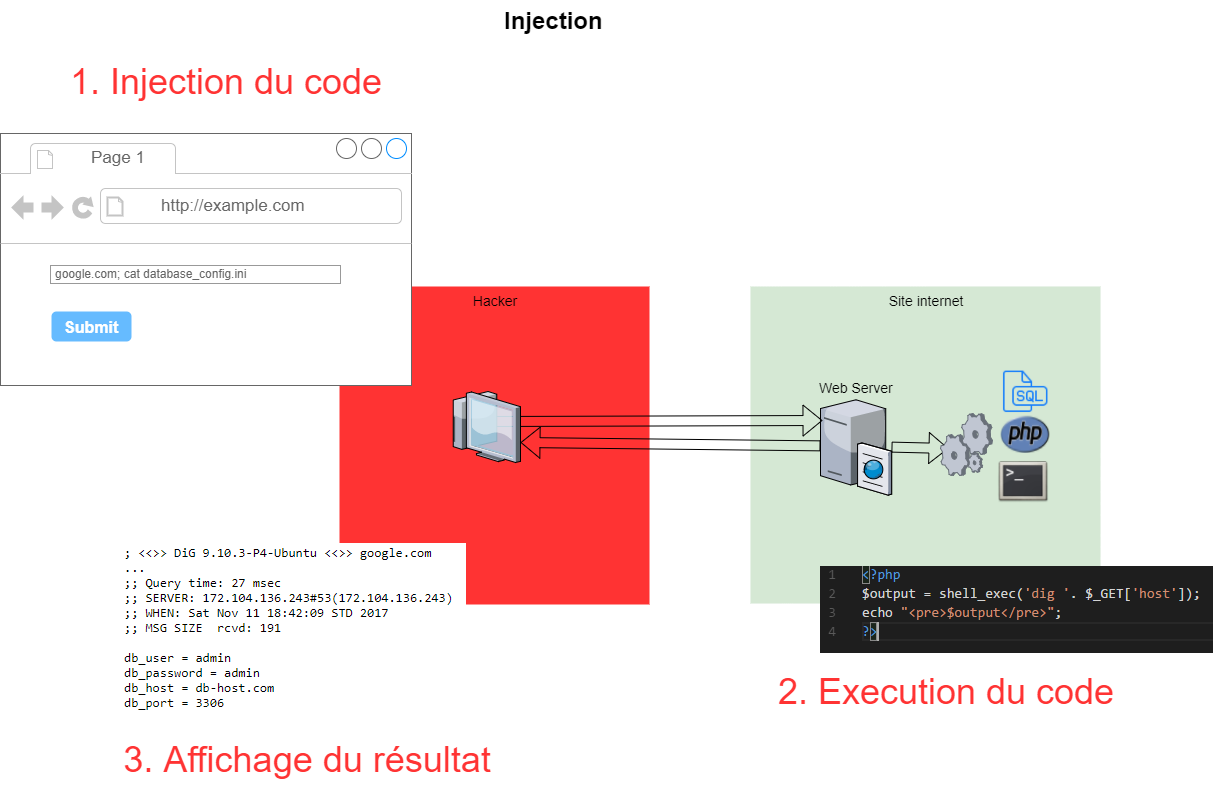
\includegraphics[width=\paperwidth]{schemas/images/injection.png}
\end{frame}
\begin{frame}{Violation de gestion d'authentification et de session}
\centering
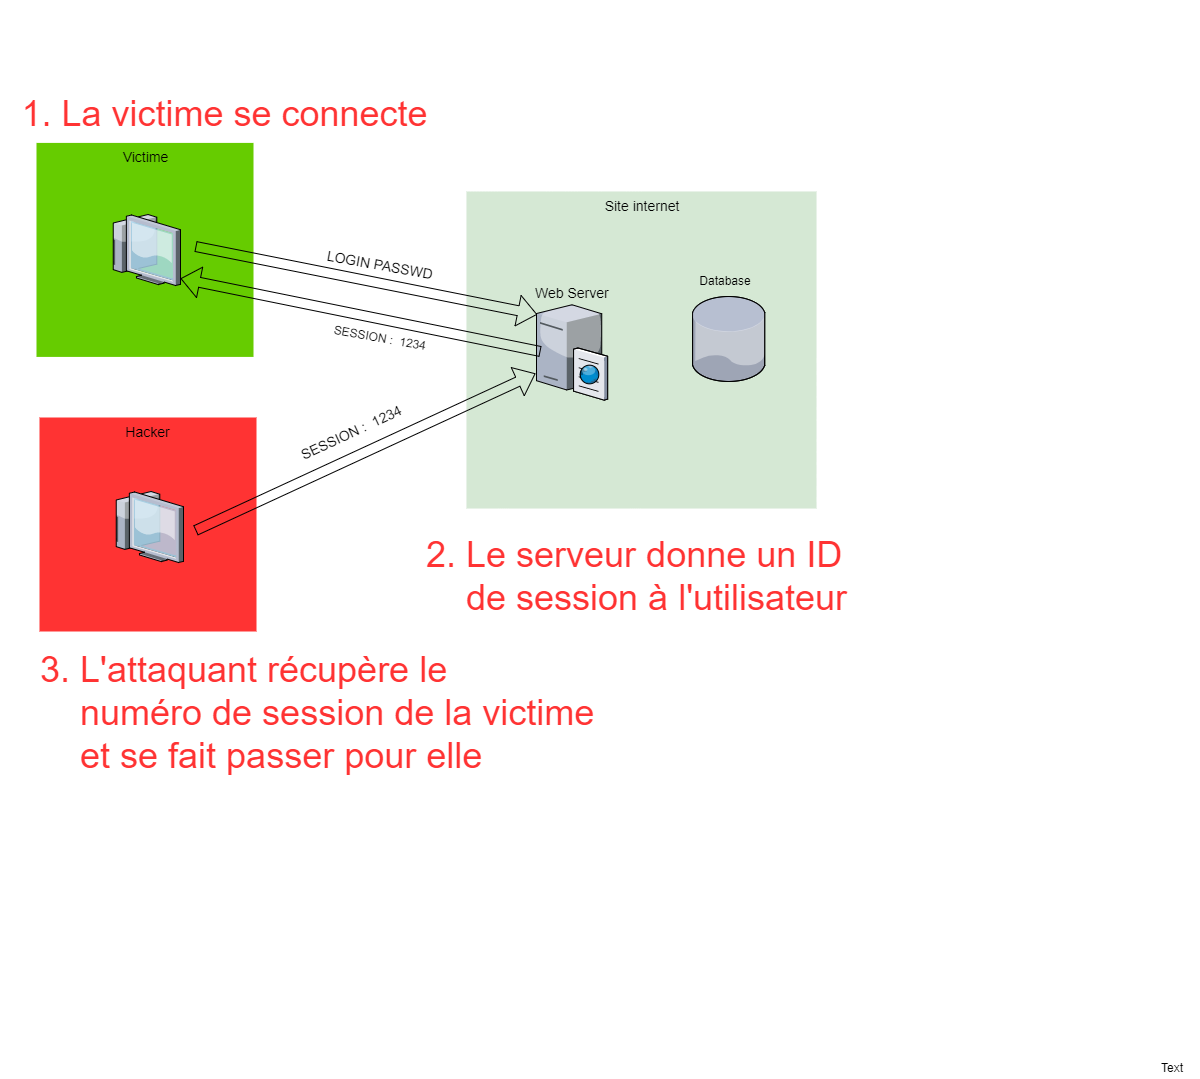
\includegraphics[width=0.95\paperwidth ]{schemas/images/broken_auth.png}
\end{frame}
\begin{frame}{Cross-Site Scripting (XSS)}
\centering
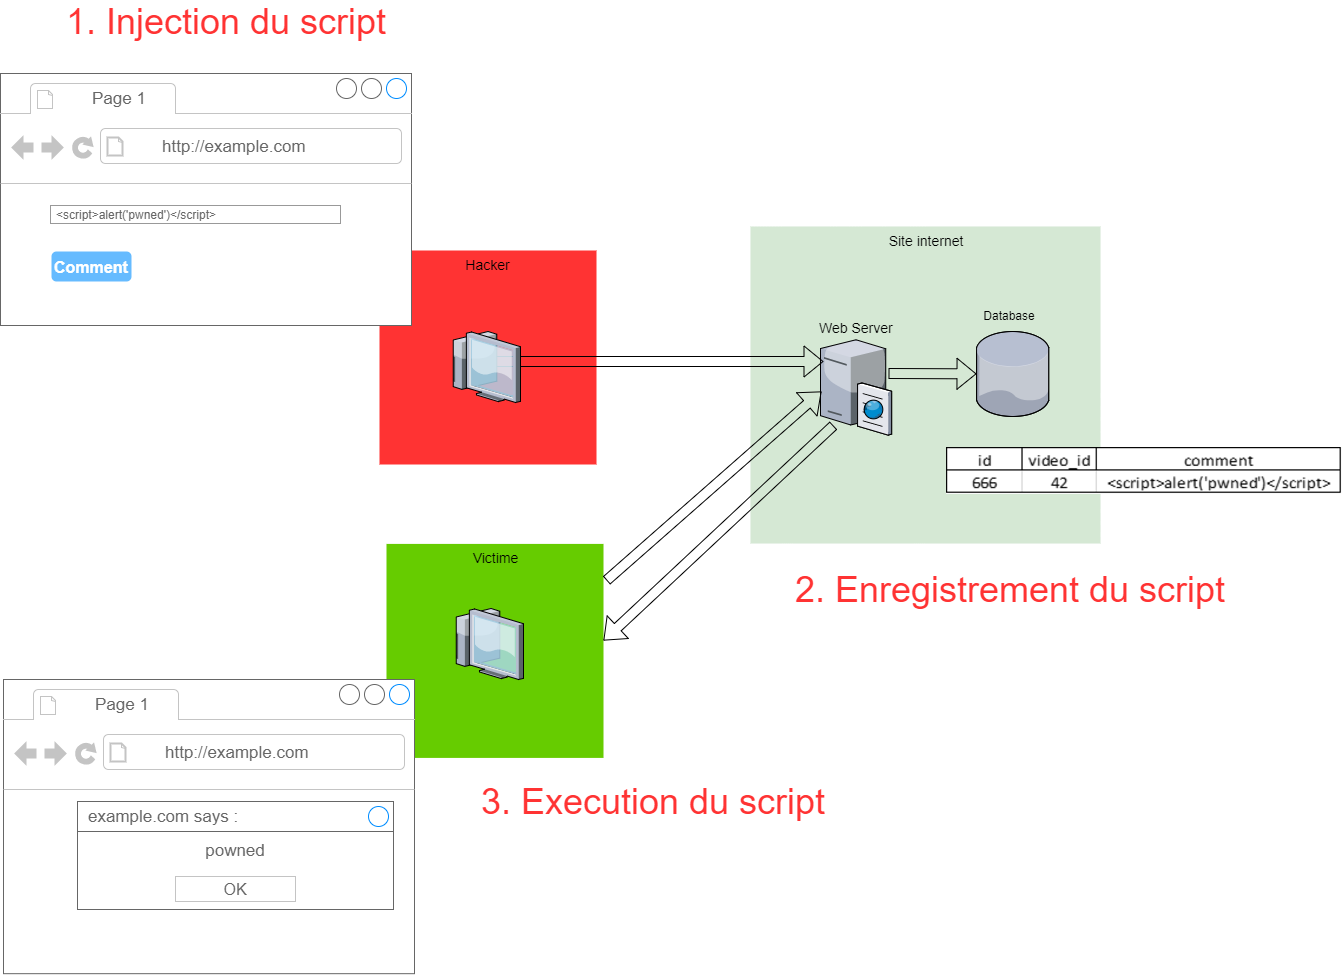
\includegraphics[width=0.92\paperwidth ]{schemas/images/XSS.png}
\end{frame}
\begin{frame}{Démonstrations}
\centering

\includegraphics[width=0.92\paperwidth ]{schemas/images/showtime.jpg}
\end{frame}

\section{Conclure un audit}	
\subsection{Elaboration du rapport d'audit} 
\begin{frame}{Elaboration du rapport d'audit}
	Audit terminé $\Rightarrow$ échéance terminée ou activités prévues réalisées
	\begin{block}{Rapport d'audit, rédigé par l'auditeur}
		\begin{itemize}
			\item Compréhensible par des non experts
			\item La liste des vulnérabilités trouvées
			\item La liste des mesures correctives proposées
			\item Déroulement des tests d'intrusion et méthodologie employés
			\item Mention des imprévues
		\end{itemize}
	\end{block}
	$\newline$
	Comment lister les vulnérabilités?
\end{frame}

\subsection{Conclusion à l'audit} 
\begin{frame}{Conclusion à l'audit}
	\begin{itemize}
		\item Réunion audité-auditeur
		\item Audité $\rightarrow$ certifier l'état de sécurité de son système
		\item Auditeur $\rightarrow$ restituer ou detruire les traces de l'audit
		\item Audit de validation ?
	\end{itemize}
\end{frame}

\begin{frame}{Conclusion}
	Audit de sécurité d'une application: 
	\begin{itemize}
		\item Nécessite du temps
		\item Sécurité $\rightarrow$ période de temps limitée
		\item Audité $\rightarrow$ bien choisir l'auditeur
	\end{itemize}
	$\newline$
	$\newline$
	Bientot remplacé par du Bug bounty?
\end{frame}
\begin{frame}{Références}
	Images: \\
	\small{\url{pixabay.com/en/brain-human-brain-knowledge-anatomy-155190/}}
	\small{\url{scanforsecurity.com/wp-content/uploads/2016/11/w3af_scanner.png}}
\end{frame}
\end{document}
